%%%%%%%%%%%%%%%%%%%%%%%%%%%%%%%%%%%%%%%%%
% Jacobs Landscape Poster
% LaTeX Template
% Version 1.0 (29/03/13)
%
% Created by:
% Computational Physics and Biophysics Group, Jacobs University
% https://teamwork.jacobs-university.de:8443/confluence/display/CoPandBiG/LaTeX+Poster
% 
% Further modified by:
% Nathaniel Johnston (nathaniel@njohnston.ca)
%
% Modified further still by:
% Abraham Nunes (nunes <at> dal <dot> ca)
%
% License:
% CC BY-NC-SA 3.0 (http://creativecommons.org/licenses/by-nc-sa/3.0/)
%
%%%%%%%%%%%%%%%%%%%%%%%%%%%%%%%%%%%%%%%%%

\documentclass[final]{beamer}

\usepackage[scale=1.24]{beamerposter} % Use the beamerposter package for laying out the poster

\usetheme{confposter} % Use the confposter theme supplied with this template

\setbeamercolor{block title}{fg=black,bg=white} % Colors of the block titles
\setbeamercolor{block body}{fg=black,bg=white} % Colors of the body of blocks
\setbeamercolor{block alerted title}{fg=white,bg=black} % Colors of the highlighted block titles
\setbeamercolor{block alerted body}{fg=black,bg=white} % Colors of the body of highlighted blocks
% Many more colors are available for use in beamerthemeconfposter.sty

%-----------------------------------------------------------
% Define the column widths and overall poster size
% To set effective sepwid, onecolwid and twocolwid values, first choose how many columns you want and how much separation you want between columns
% In this template, the separation width chosen is 0.024 of the paper width and a 4-column layout
% onecolwid should therefore be (1-(# of columns+1)*sepwid)/# of columns e.g. (1-(4+1)*0.024)/4 = 0.22
% Set twocolwid to be (2*onecolwid)+sepwid = 0.464
% Set threecolwid to be (3*onecolwid)+2*sepwid = 0.708

\newlength{\sepwid}
\newlength{\onecolwid}
\newlength{\twocolwid}
\newlength{\threecolwid}
\setlength{\paperwidth}{48in} % A0 width: 46.8in
\setlength{\paperheight}{36in} % A0 height: 33.1in
\setlength{\sepwid}{0.024\paperwidth} % Separation width (white space) between columns
\setlength{\onecolwid}{0.22\paperwidth} % Width of one column
\setlength{\twocolwid}{0.464\paperwidth} % Width of two columns
\setlength{\threecolwid}{0.708\paperwidth} % Width of three columns
\setlength{\topmargin}{-0.5in} % Reduce the top margin size
%-----------------------------------------------------------

\usepackage{graphicx}  % Required for including images

\usepackage{booktabs} % Top and bottom rules for tables

\title{Estimates of COVID-19 Excess Deaths in New Zealand that Properly Account for Demographic Trends}

\author{John Bryant$^1$, Kim Dunstan$^2$, Pubudu Senanayake$^2$, Lucianne Varn$^2$, and Junni Zhang$^3$}

\institute{$^{1}$Bayesian Demography Limited, $^{2}$Statistics New Zealand, $^{3}$Peking University}

%----------------------------------------------------------------------------------------

\begin{document}

\addtobeamertemplate{block end}{}{\vspace*{2ex}} % White space under blocks
\addtobeamertemplate{block alerted end}{}{\vspace*{2ex}} % White space under highlighted (alert) blocks

\setlength{\belowcaptionskip}{2ex} % White space under figures
\setlength\belowdisplayshortskip{2ex} % White space under equations

\begin{frame}[t] % The whole poster is enclosed in one beamer frame

\begin{columns}[t] % The whole poster consists of three major columns, the second of which is split into two columns twice - the [t] option aligns each column's content to the top

\begin{column}{\sepwid}\end{column} % Empty spacer column

\begin{column}{\onecolwid} % The first column


\setbeamercolor{block alerted title}{fg=white,bg=dalgrey} % Change the alert block title colors
\setbeamercolor{block alerted body}{fg=black,bg=white} % Change the alert block body colors

\begin{alertblock}{Objectives}

Obtain new estimates for excess deaths in Aotearoa New Zealand during the COVID-19 epidemic that
\begin{itemize}
\item account for differences by age, sex, and season,
\item include measures of uncertainty, and
\item are easy to replicate.
\end{itemize}

\end{alertblock}


\begin{block}{Background}

  \begin{itemize}
  \item New Zealand closed borders and imposed strict lockdowns during COVID-19
  \item Debate over number of excess deaths
  \item Existing estimates do not properly account for demographic trends, e.g.  age-sex differentials, pre-existing trends, seasonal effects, population change
 \end{itemize}

\end{block}


  \begin{block}{Data}

\begin{itemize}
\item Population by 5-year age group, sex, month, 1998--2023, from Statistics New Zealand
\item Deaths by 5-year age group, sex, month, 1998--2023, from Statistics New Zealand
\end{itemize}

\end{block}

\begin{block}{Statistical model}

\begin{figure}
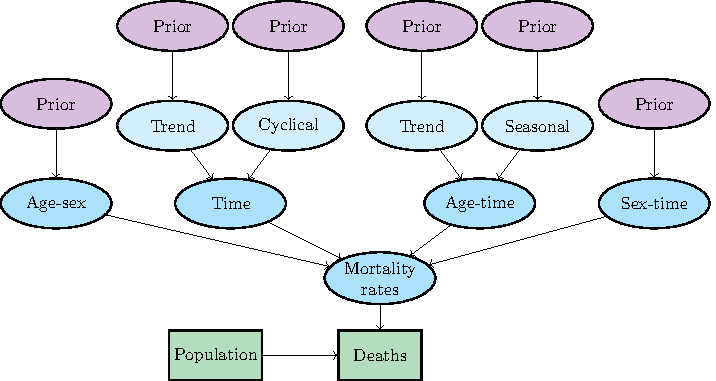
\includegraphics[width = 0.95 \linewidth]{dag.pdf}
\caption{Bayesian hierarchical model used for estimation and forecasting}
\end{figure}

\end{block}

%----------------------------------------------------------------------------------------

\end{column} % End of the first column

\begin{column}{\sepwid}\end{column} % Empty spacer column

\begin{column}{\twocolwid} % Begin a column which is two columns wide (column 2)

  \begin{columns}[t,totalwidth=\twocolwid] % Split up the two columns wide column

\begin{column}{\onecolwid}\vspace{-.6in} % The first column within column 2 (column 2.1)

\begin{block}{Forecasts of rates}
\begin{figure}
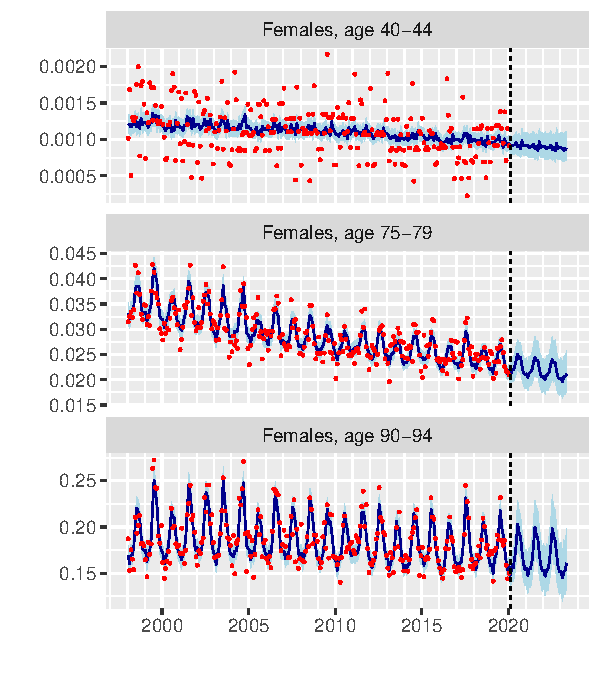
\includegraphics[width = \linewidth]{fig_forecasted_rates}
\caption{Estimates and forecasts of mortality rates for selected groups. Blue lines and bands are point estimates and 95\% credible intervals from model. Red dots are direct estimates.}
\end{figure}
\end{block}

\end{column} % End of column 2.1

\begin{column}{\onecolwid}\vspace{-.6in} % The second column within column 2 (column 2.2)

\begin{block}{Excess Deaths by Age}
\begin{figure}
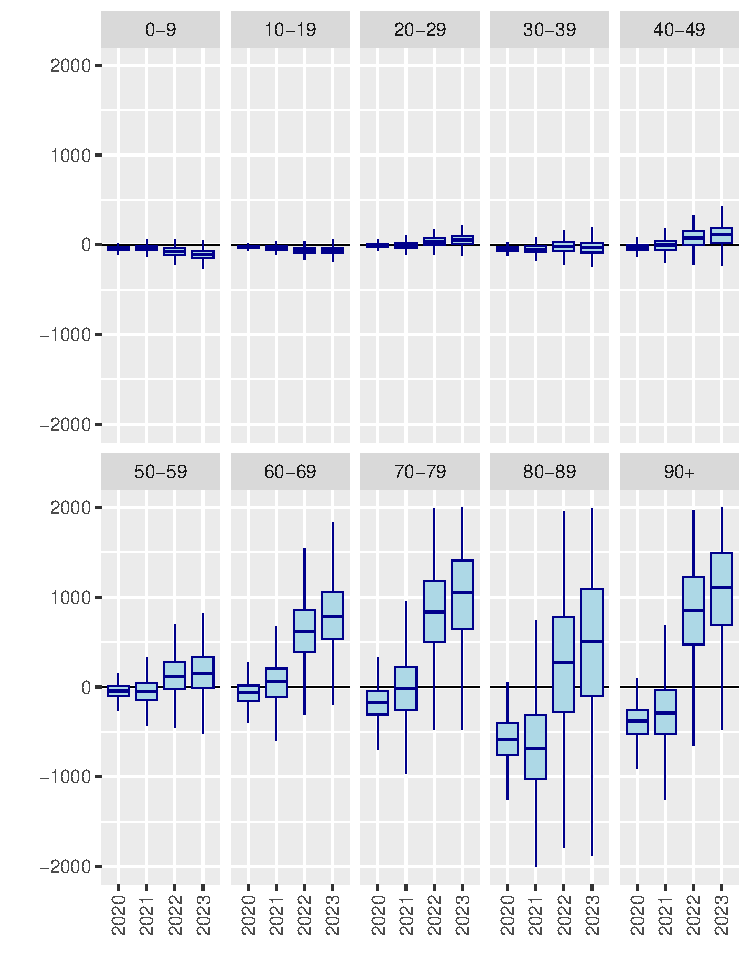
\includegraphics[width = 0.9 \linewidth]{fig_excess_age}
\caption{Excess deaths, by age group, by year}
\end{figure}
\end{block}

\end{column} % End of column 2.2

\end{columns} % End of the split of column 2 - any content after this will now take up 2 columns width


\setbeamercolor{block alerted title}{fg=black,bg=dalgold} % Change the alert block title colors
\setbeamercolor{block alerted body}{fg=black,bg=white} % Change the alert block body colors

\begin{alertblock}{Excess Deaths}

\begin{figure}
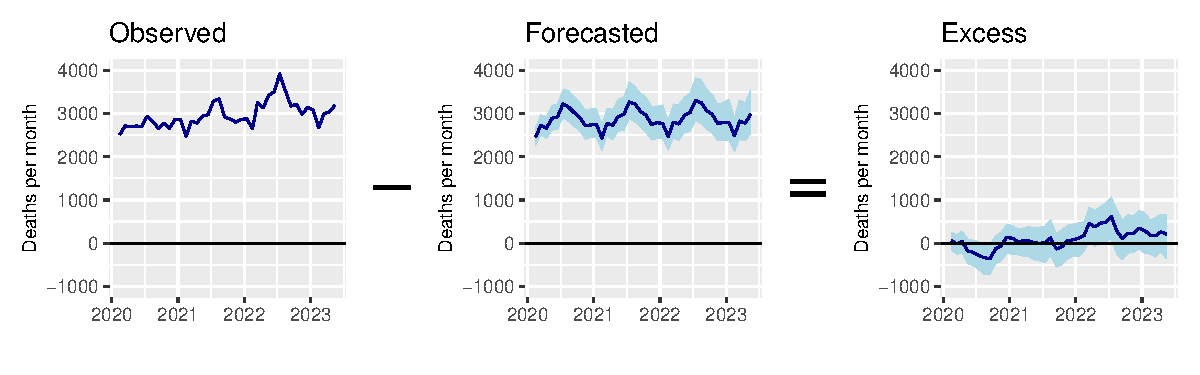
\includegraphics[width = \linewidth]{fig_calc_excess}
\caption{Calculation of monthly excess deaths: forecasted deaths are subtracted from actual deaths}
\end{figure}

\end{alertblock} 

\end{column} % End of the second column

\begin{column}{\sepwid}\end{column} % Empty spacer column

\begin{column}{\onecolwid} % The third column

\begin{block}{Life expectancy}
\begin{figure}
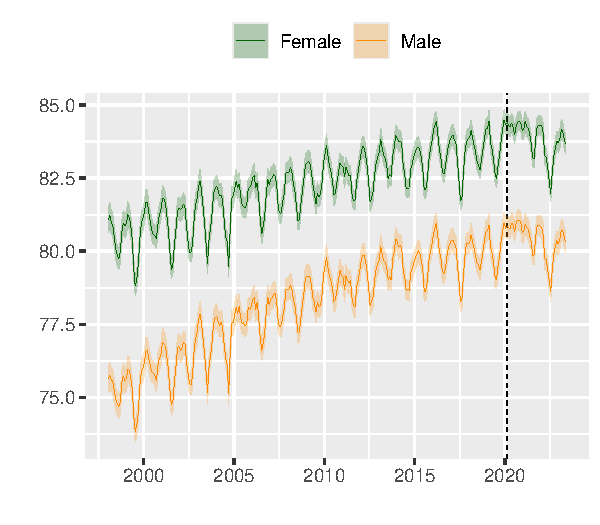
\includegraphics[width = 0.95\linewidth]{fig_lifeexp}
\caption{Estimates of life expectancy at birth, from model fitted to data for 1998--2023}
\end{figure}
\end{block}

  
\begin{block}{Conclusion}
  \begin{itemize}
  \item Monthly excess deaths between -500 and 1000
  \item Annual excess deaths in 2022--2023 higher than 2020--2021
  \item Excess deaths concentrated among older people
  \end{itemize}
\end{block}

\begin{block}{Notes}
\begin{itemize}
\item Work in progress, and results are provisional
\item Statistical models implemented using R package \textbf{bage}
\end{itemize}
\end{block}

\setbeamercolor{block alerted title}{fg=black,bg=dalblue} % Change the alert block title colors
\setbeamercolor{block alerted body}{fg=black,bg=white} % Change the alert block body colors

\begin{alertblock}{Contact Information}
  john@bayesiandemography.com
  kim.dunstan@stats.govt.nz
\end{alertblock}

%----------------------------------------------------------------------------------------

\end{column} % End of the third column

\end{columns} % End of all the columns in the poster

\end{frame} % End of the enclosing frame

\end{document}
